%%%%%%%%%%%%%%%%%%%%%%%%%%%%%%% main.tex %%%%%%%%%%%%%%%%%%%%%%%%%%%%%%%
%                                                                      %
% --------------------- Report Template IST [EN] --------------------- %
%                                                                      %
%       João Marafuz Gaspar                                           %
%       Departamento de Engenharia Eletrotécnica e de Computadores     %
%       Instituto Superior Tecnico                                     %
%       Av. Rovisco Pais                                               %
%       1049-001 Lisboa                                                %
%       Portugal                                                       %
%       E-mail: joao.marafuz.gaspar@tecnico.ulisboa.pt                 %
%                                                                      %
%  Created:       Jul 30, 2022                                         %
%  Last Modified: May 18, 2024                                         %
%                                                                      %
%%%%%%%%%%%%%%%%%%%%%%%%%%%%%%%%%%%%%%%%%%%%%%%%%%%%%%%%%%%%%%%%%%%%%%%%
%  Revision history                                                    %
%  v1 - 2022/07/30 - original template                                 %
%  v2 - 2023/04/06 - change superscript in the cover, updated font,    %
%                    added subfigures and table                        %
%  v3 - 18/05/2024 - update for using only one font, known by the name %
%                    of CMU Serif Roman                                %
%%%%%%%%%%%%%%%%%%%%%%%%%%%%%%%%%%%%%%%%%%%%%%%%%%%%%%%%%%%%%%%%%%%%%%%%
%                              Preamble                                %
%%%%%%%%%%%%%%%%%%%%%%%%%%%%%%%%%%%%%%%%%%%%%%%%%%%%%%%%%%%%%%%%%%%%%%%%

% ----------------------------------------------------------------------
% Set the document class
% ----------------------------------------------------------------------
\documentclass[12pt]{article}

% ----------------------------------------------------------------------
% Define external packages, language, margins, fonts, new commands 
% and colors
% ----------------------------------------------------------------------
\usepackage[utf8]{inputenc} % Codification
\usepackage[english]{babel} % Writing idiom

\usepackage[export]{adjustbox} % Align images
\usepackage{amsmath} % Extra commands for math mode
\usepackage{amssymb} % Mathematical symbols
\usepackage{anysize} % Personalize margins
    \marginsize{2cm}{2cm}{2cm}{2cm} % {left}{right}{above}{below}
\usepackage{appendix} % Appendices
\usepackage{cancel} % Expression cancellation
\usepackage{caption} % Captions
    \captionsetup{labelfont={bf}}
\usepackage{cite} % Citations, like [1 - 3]
\usepackage{color} % Text coloring
\usepackage{fancyhdr} % Head note and footnote
    \pagestyle{fancy}
    \fancyhf{}
    \fancyhead[L]{\footnotesize \today} % Left of Head note
    \fancyhead[R]{\footnotesize Piyush Acharya} % Right of Head note
    \fancyfoot[L]{\footnotesize P4 AP/IB Physics 1} % Left of Footnote
    \fancyfoot[C]{\thepage} % Center of Footnote
    \fancyfoot[R]{\footnotesize Momentum Lab} % Right of Footnote
    \renewcommand{\footrulewidth}{0.4pt} % Footnote rule
\usepackage{float} % Utilization of [H] in figures
\usepackage{graphicx} % Figures in LaTeX
\usepackage[colorlinks = true, plainpages = true, linkcolor = istblue, urlcolor = istblue, citecolor = istblue, anchorcolor = istblue]{hyperref}
\usepackage{indentfirst} % First paragraph
\usepackage[super]{nth} % Superscripts
\usepackage{siunitx} % SI units
\usepackage{subcaption} % Subfigures
\usepackage{titlesec} % Font
    \titleformat{\section}{\Large\bfseries}{\thesection}{1em}{}
    \titleformat{\subsection}{\large\bfseries}{\thesubsection}{1em}{}
    \titleformat{\subsubsection}{\normalsize\bfseries}{\thesubsubsection}{1em}{}
    \fancyfoot[C]{\thepage}

% Random text (not needed)
\usepackage{lipsum}
\usepackage{duckuments}

% New and re-newcommands
\newcommand{\sen}{\operatorname{\sen}} % Sine function definition
\newcommand{\HRule}{\rule{\linewidth}{0.5mm}} % Specific rule definition
\renewcommand{\appendixpagename}{\LARGE Appendices}

% Colors
\definecolor{istblue}{RGB}{3, 171, 230}
\definecolor{dkgreen}{rgb}{0,0.6,0}
\definecolor{gray}{rgb}{0.5,0.5,0.5}

%%%%%%%%%%%%%%%%%%%%%%%%%%%%%%%%%%%%%%%%%%%%%%%%%%%%%%%%%%%%%%%%%%%%%%%%
%                                 Document                             %
%%%%%%%%%%%%%%%%%%%%%%%%%%%%%%%%%%%%%%%%%%%%%%%%%%%%%%%%%%%%%%%%%%%%%%%%
\begin{document}

% ----------------------------------------------------------------------
% Cover
% ----------------------------------------------------------------------
\begin{center}
    \begin{figure}
        \vspace{-1.0cm}
        
\includegraphics[scale = 0.3, left]{Images/IST_B.png} % IST logo
    \end{figure}
    \mbox{}\\[2.0cm]
    \textsc{\Huge AP/IB Physics 1}\\[2.5cm]
    \textsc{\LARGE Period 4}\\[2.0cm]
    \HRule\\[0.4cm]
    {\large \bf {Momentum Lab}}\\[0.2cm]
    \HRule\\[1.5cm]
\end{center}

\begin{flushleft}
    \textbf{Authors:}
\end{flushleft}

\begin{center}
    \begin{minipage}{0.5\textwidth}
        \begin{flushleft}
            Piyush Acharya\\
        \end{flushleft}
    \end{minipage}%
    \begin{minipage}{0.5\textwidth}
        \begin{flushright}
            \href{mailto:hey@piyushacharya.com}{\texttt{hey@piyushacharya.com}}\\
        \end{flushright}
    \end{minipage}
\end{center}
    
\begin{center}
    \large \bf 2023/2024 -- \nth{2} Semester, P4
\end{center}

\thispagestyle{empty}

\setcounter{page}{0}

\newpage

% ----------------------------------------------------------------------
% Contents
% ----------------------------------------------------------------------
\tableofcontents 

\newpage

% ----------------------------------------------------------------------
% Body
% ----------------------------------------------------------------------
\section{Objective}

\lipsum[1] \cite{refs1}

\section{Problem exposition} 

\lipsum[1] \cite{refs2}

\lipsum[2-3]

\newpage

\section{Solution presentation}

\subsection{How to present figures}

\subsubsection{How to present just one figure}

\begin{figure}[H]
	\begin{center}
 		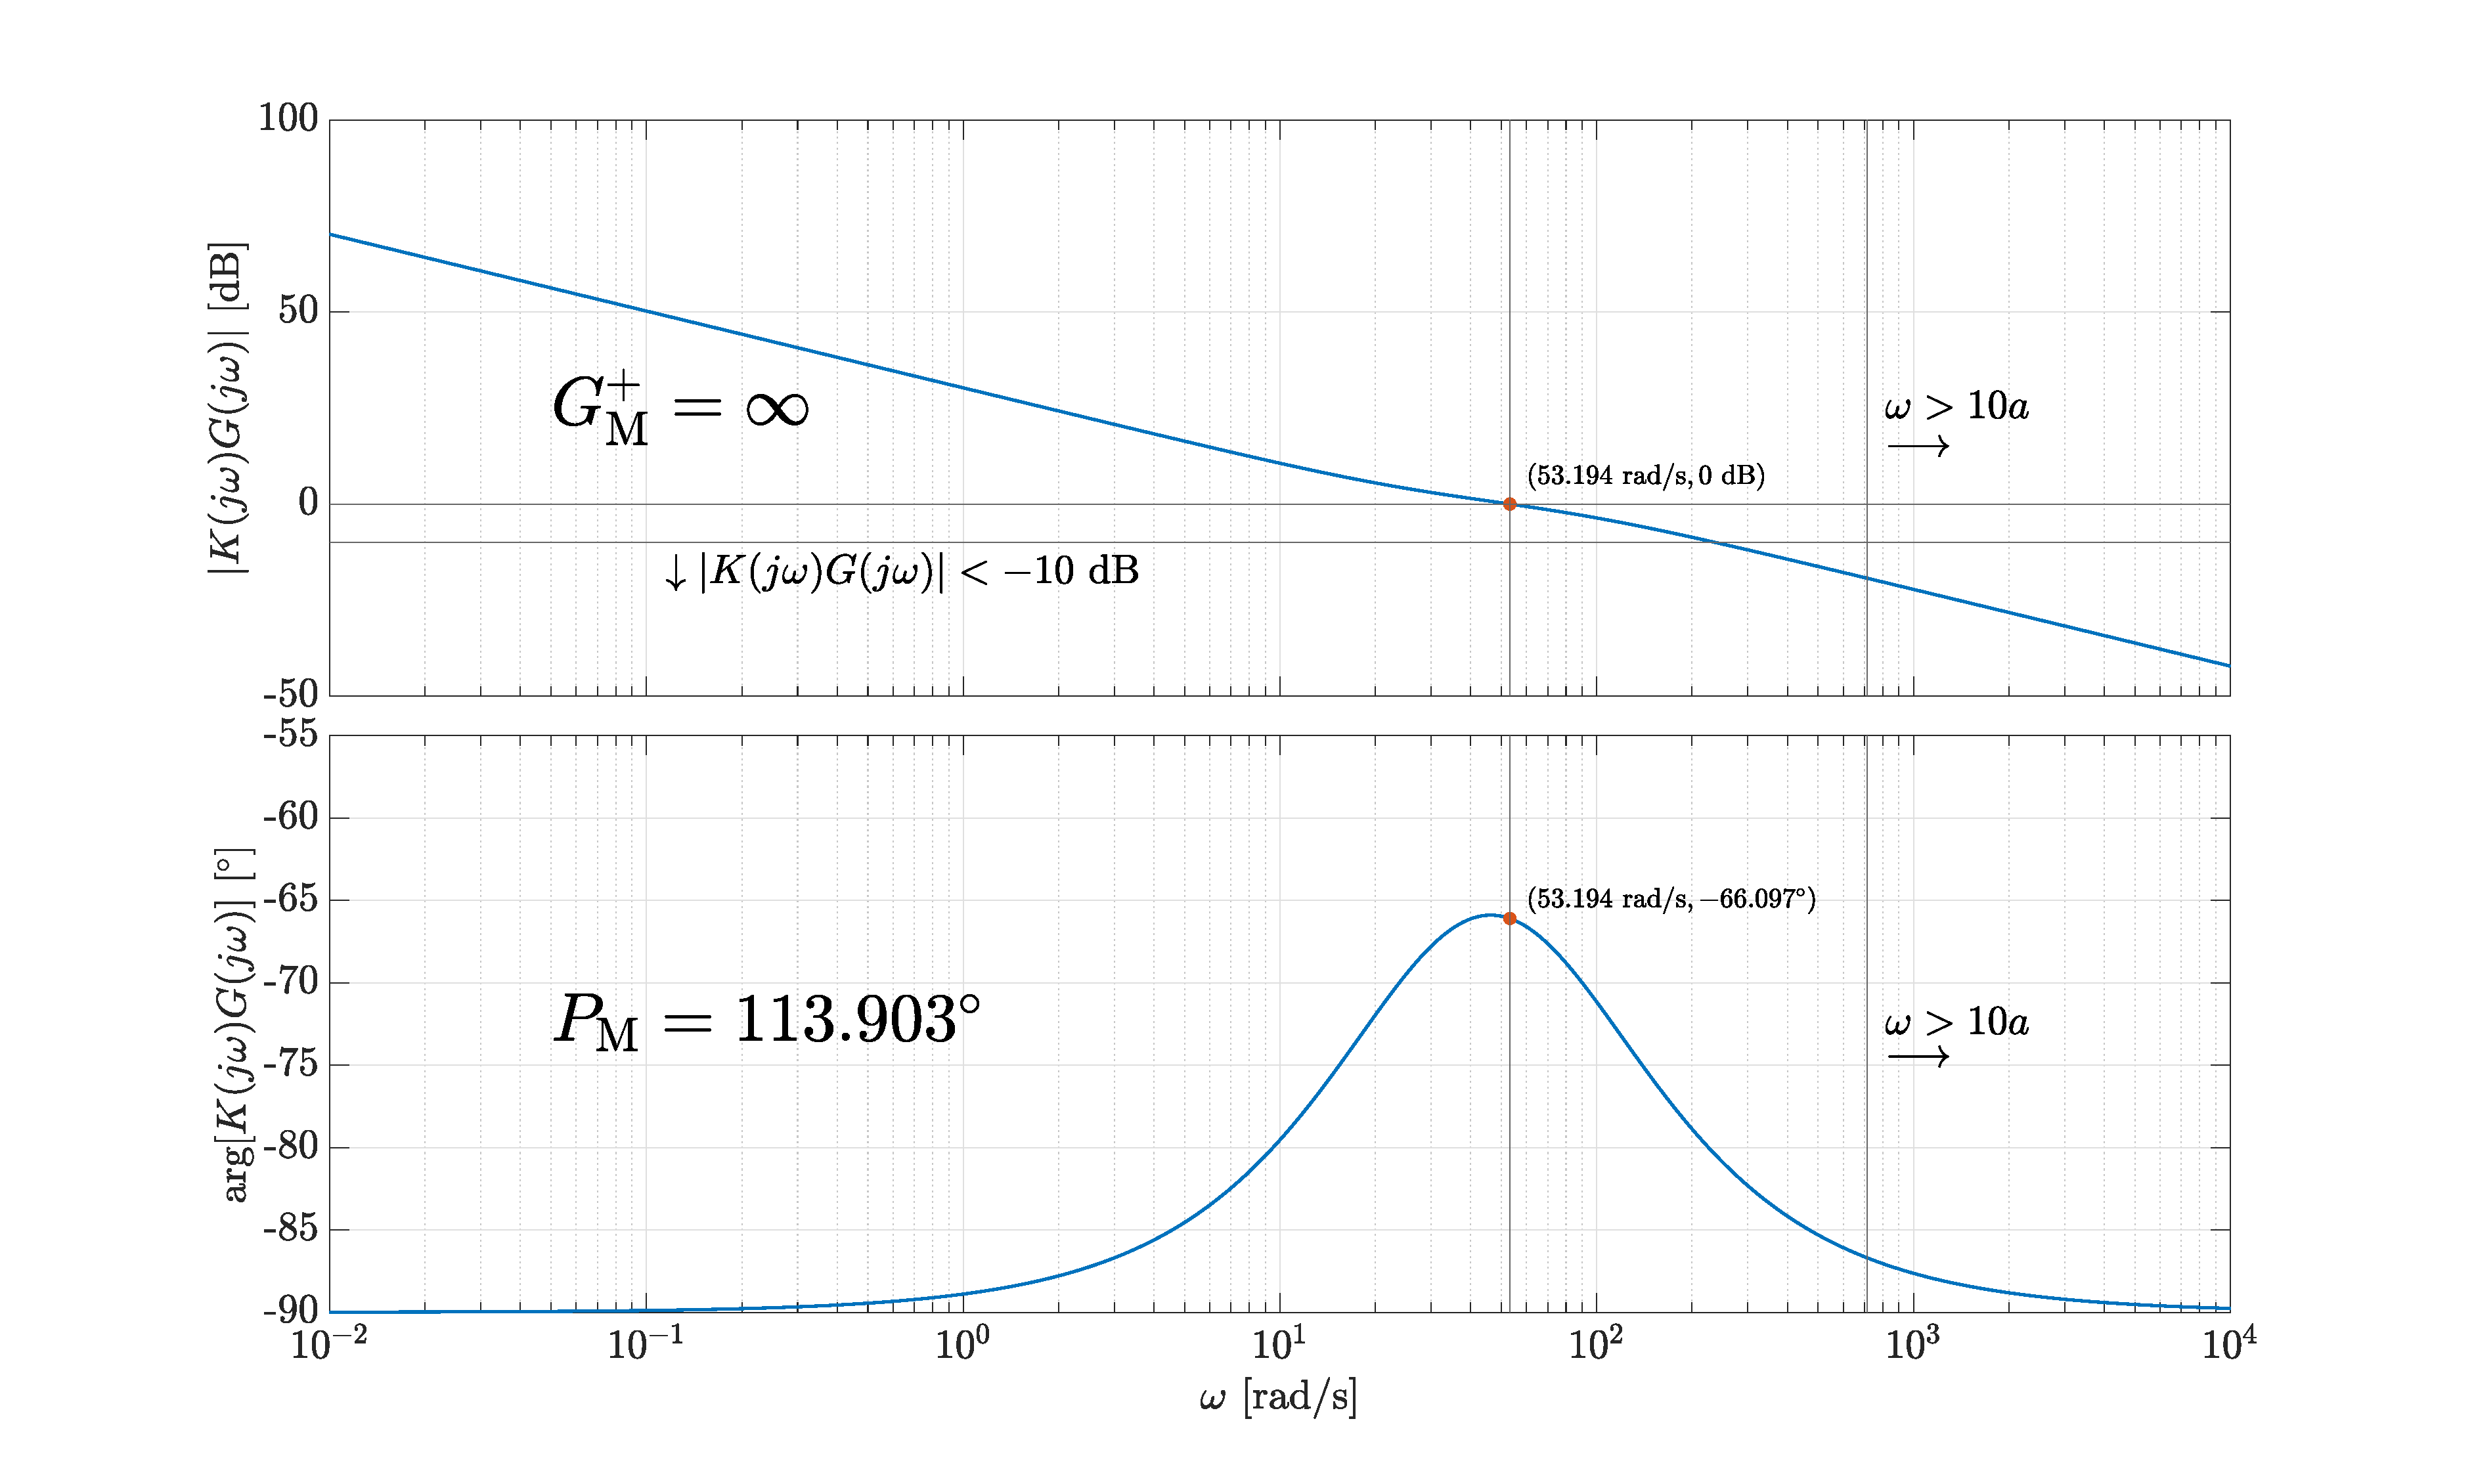
\includegraphics[width = 0.8\textwidth]{Images/Image.eps}
 		\caption{Caption}
 		\label{fig:1}
	\end{center} 
\end{figure}

\subsubsection{How to present subfigures}

\begin{figure}[H]
    \centering
    \begin{subfigure}{0.33\textwidth}
        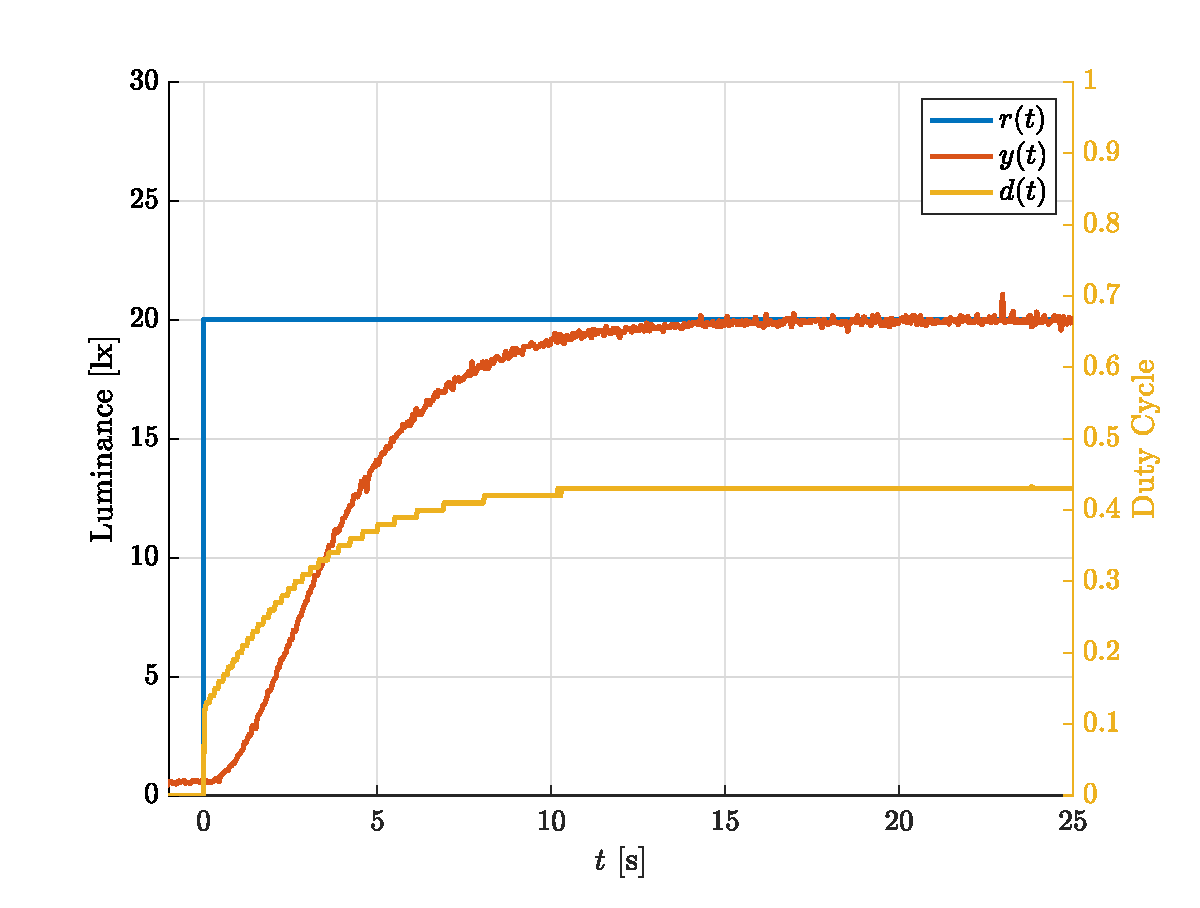
\includegraphics[width=\linewidth]{Images/Subimage1.eps}
        \caption{Subfigure 1}
        \label{fig:2.1}
    \end{subfigure}%
    \begin{subfigure}{0.33\textwidth}
        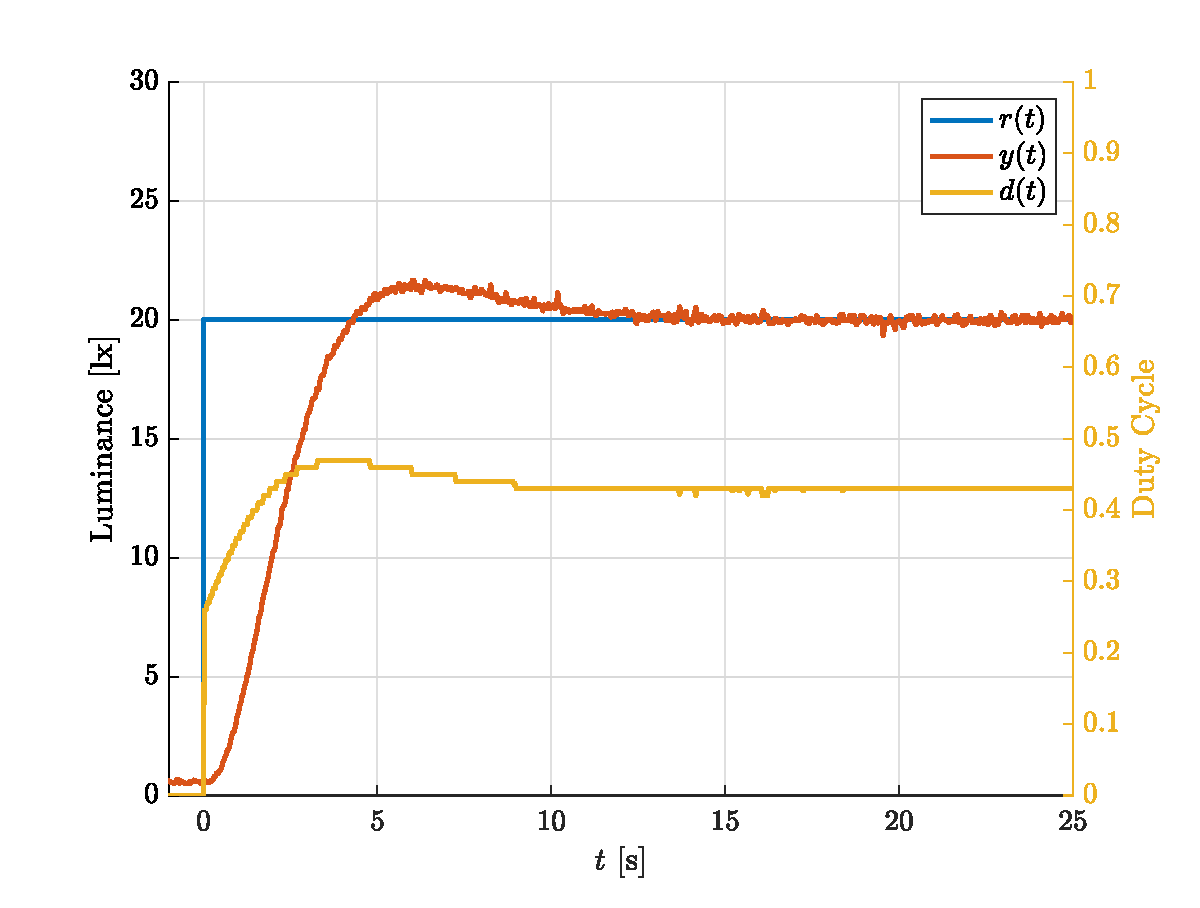
\includegraphics[width=\linewidth]{Images/Subimage2.eps}
        \caption{Subfigure 2}
        \label{fig:2.2}
    \end{subfigure}%
    \begin{subfigure}{0.33\textwidth}
        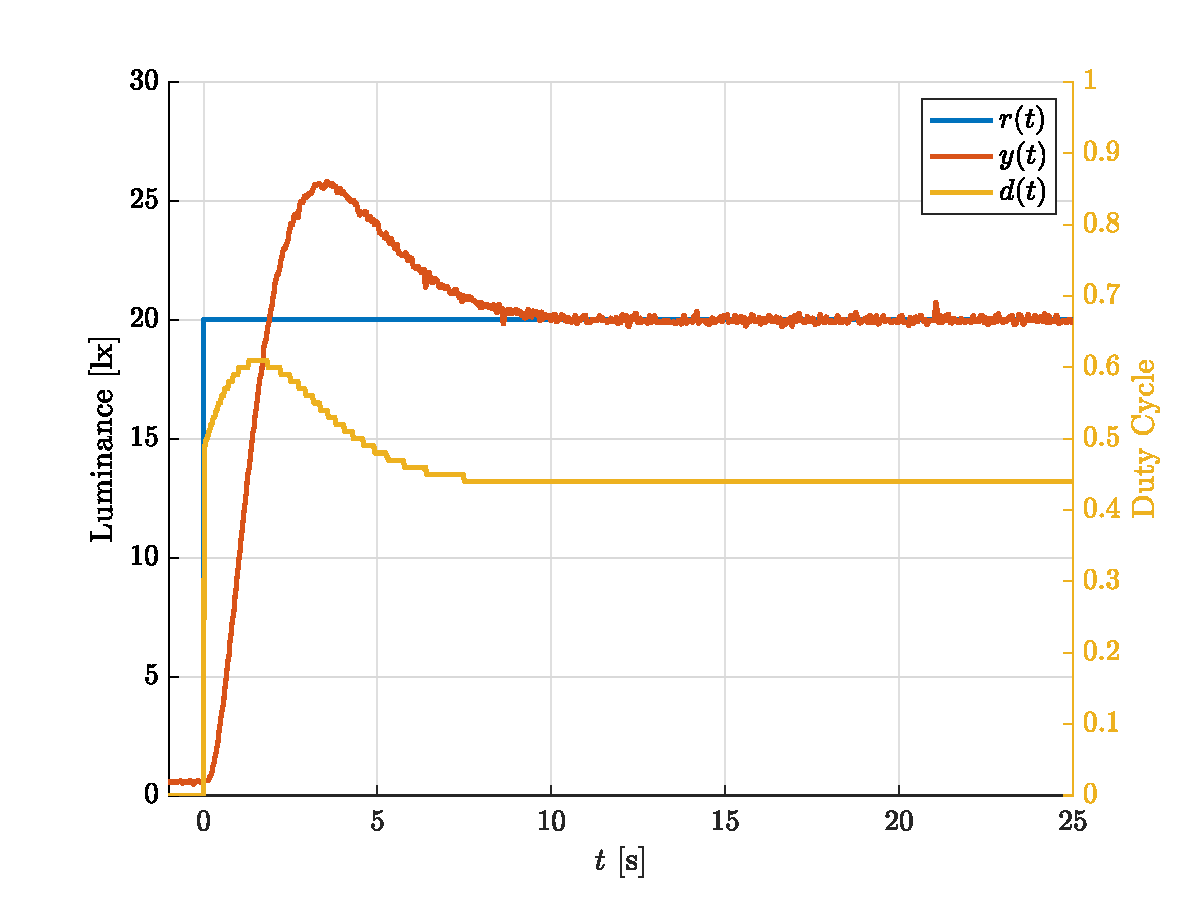
\includegraphics[width=\linewidth]{Images/Subimage3.eps}
        \caption{Subfigure 3}
        \label{fig:2.3}
    \end{subfigure}
    \caption{Caption}
    \label{fig:2}
\end{figure}

\subsection{How to present a table}

\begin{table}[H]
    \centering
    \caption{Orbital parameters for Constellation II}
    \label{tab:1}
    \begin{tabular}{|c|c|c|c|c|c|c|}
        \hline
        Satellite & $a \ [\SI{}{\meter}]$ & $e$  & $T_0$                 & $\varpi \ [\SI{}{\degree}]$ & $\Omega \ [\SI{}{\degree}]$ & $i \ [\SI{}{\degree}]$ \\ \hline
        1        & 20427.093             & 0.1 & $t_0$                 & 270                          & 0         & 60    \\ \hline
        2        & 20427.093             & 0.1 & $t_0 + \frac{T}{2}$   & 90                           & 240       & 60    \\ \hline
        3 (stat.) & 20427.093             & 0 &  N/A (circular orbit)  &  N/A (circular orbit)       & 67        & 0    \\ \hline
        4 (stat.) & 20427.093             & 0    & N/A (circular orbit) & N/A (circular orbit)       & 207       & 0     \\ \hline
    \end{tabular}
\end{table}

\subsection{How to present an equation}

\begin{equation}
    u(\lambda,T)=\frac{8\pi hc\lambda^{-5}}{e^{hc/\lambda kT}-1}
    \label{eq:1}
\end{equation}

% ----------------------------------------------------------------------
% Conclusion
% ----------------------------------------------------------------------
\section{Conclusion}

\lipsum[1] \cite{refs1, refs2, refs3}

% ----------------------------------------------------------------------
% References
% ----------------------------------------------------------------------
\bibliographystyle{plain}
\bibliography{refs}

% ----------------------------------------------------------------------
% Appendices
% ----------------------------------------------------------------------
\appendix  
\clearpage
\addappheadtotoc 
\appendixpage 

\section{First appendix}

\lipsum[1]

\section{Second appendix}

\lipsum[1]
\end{document}